\documentclass[letter]{article}

\usepackage[english]{babel}
\usepackage[utf8]{inputenc}
\usepackage{amsmath}
\usepackage[colorinlistoftodos]{todonotes}
\usepackage{makecell}
\usepackage{multirow}
\usepackage{caption}
\usepackage{subcaption}
\usepackage{graphicx}
\usepackage{hyperref}
\usepackage{float}
\usepackage[all]{hypcap}
\usepackage[space]{grffile}
\usepackage{enumitem}
\usepackage{bm}
\usepackage{bbm}
\usepackage{algorithm}
\usepackage{algorithmic}
\usepackage{nccmath, mathtools}
\usepackage{amsthm,amssymb}
\usepackage{listings}

\newlist{questions}{enumerate}{1}
\setlist[questions, 1]{label = \arabic*}
\newlist{bonus}{enumerate}{1}
\setlist[bonus, 1]{label = Bonus \arabic*}

\definecolor{mygreen}{rgb}{0,0.6,0}
\definecolor{mygray}{rgb}{0.5,0.5,0.5}
\definecolor{mymauve}{rgb}{0.58,0,0.82}

\lstset{ 
	backgroundcolor=\color{white},   % choose the background color; you must add \usepackage{color} or \usepackage{xcolor}; should come as last argument
	basicstyle=\footnotesize,        % the size of the fonts that are used for the code
	breakatwhitespace=false,         % sets if automatic breaks should only happen at whitespace
	breaklines=true,                 % sets automatic line breaking
	captionpos=b,                    % sets the caption-position to bottom
	commentstyle=\color{mygreen},    % comment style
	deletekeywords={...},            % if you want to delete keywords from the given language
	escapeinside={\%*}{*)},          % if you want to add LaTeX within your code
	extendedchars=true,              % lets you use non-ASCII characters; for 8-bits encodings only, does not work with UTF-8
	frame=single,	                   % adds a frame around the code
	keepspaces=true,                 % keeps spaces in text, useful for keeping indentation of code (possibly needs columns=flexible)
	keywordstyle=\color{blue},       % keyword style
	language=Octave,                 % the language of the code
	morekeywords={*,...},            % if you want to add more keywords to the set
	numbers=left,                    % where to put the line-numbers; possible values are (none, left, right)
	numbersep=5pt,                   % how far the line-numbers are from the code
	numberstyle=\tiny\color{mygray}, % the style that is used for the line-numbers
	rulecolor=\color{black},         % if not set, the frame-color may be changed on line-breaks within not-black text (e.g. comments (green here))
	showspaces=false,                % show spaces everywhere adding particular underscores; it overrides 'showstringspaces'
	showstringspaces=false,          % underline spaces within strings only
	showtabs=false,                  % show tabs within strings adding particular underscores
	stepnumber=2,                    % the step between two line-numbers. If it's 1, each line will be numbered
	stringstyle=\color{mymauve},     % string literal style
	tabsize=2,	                   % sets default tabsize to 2 spaces
	title=\lstname                   % show the filename of files included with \lstinputlisting; also try caption instead of title
}

% Adjust margins
\addtolength{\oddsidemargin}{-0.75in}
\addtolength{\evensidemargin}{-0.75in}
\addtolength{\textwidth}{1.5in}
\addtolength{\topmargin}{-.5in}
\addtolength{\textheight}{1.5in}
\setlength\parindent{0pt}
\setlength{\parskip}{5pt}

\title{CS 520: Assignment 4 - Colorization}
\author{Haoyang Zhang, Han Wu, Shengjie Li, Zhichao Xu}
\date{\today}

\begin{document}
\maketitle

\section{Introduction, group members and division of workload}
\label{sec:Introduction}

In this group project, we implemented a image colorizer which can generate satisfying color images given grayscale images. \\
\begin{tabular}{| p{2.5cm} | p{\textwidth -3.5cm} |}
	\hline
	\makecell[c]{Name \\ RUID} & Workload \\
	\hline
	\makecell[c]{Haoyang Zhang \\ 188008687} & {Implemented a toy CNN based on numpy. Wrote Usage.html and HowToBuildACNN.html which are two documents about the toy CNN.} \\
	\hline
	\makecell[c]{Han Wu \\ 189008460} & {Wrote part of the report and participated in the discussion. Analyzed the outcome of our colorizer.} \\
	\hline
	\makecell[c]{Shengjie Li \\ 188008047} & {Implemented the colorizer. Trained the model. Wrote part of the report. Finished the format design of the report using \LaTeX. } \\
	\hline
	\makecell[c]{Zhichao Xu \\ 188008912} & {Wrote part of the report. Came up with the original structure of network.} \\
	\hline
\end{tabular}


\section{The Problem}
\label{sec:The Problem}
\begin{itemize}
	\item {\textbf{Representing the Process:}   } 
	\begin{enumerate}
		\item {\textbf{How can you represent the coloring process in a way that a computer can handle?}}
		\par{A color image can be interpreted as an array with 3 channels -- channel R,  channel G, channel B. A grayscale image can be interpreted as a color image being compressed to having only one channel gray, by the formula $ Gray(r, g, b) = 0.21r + 0.72g + 0.07b $. So the coloring process can be seen as: given a one-channel image, produce a three-channel image. To achieve this, we are using a CNN with autoencoder.}
		\item {\textbf{What spaces are you mapping between? What maps do you want to consider?} Note that mapping
			from a single grayscale value gray to a corresponding color (r, g, b) on a pixel by pixel basis, you do not have
			enough information in a single gray value to reconstruct the correct color (usually).}
	\end{enumerate}
	\item {\textbf{Data:}} 
	\begin{enumerate}
		\item {\textbf{Where are you getting your data from to train/build your model?}}
		\par{We are using the \href{http://www.cs.toronto.edu/~kriz/cifar.html}{The CIFAR-10 dataset}.}
		\par{This dataset consists of 60,000 $ 32\times32 $ colour images in 10 classes, with 6,000 images per class. There are 50,000 training images and 10,000 test images in total. The dataset is divided into five training batches and one test batch, each with 10,000 images. The test batch contains exactly 1,000 randomly-selected images from each class. }
		\begin{figure}[H]
			\centering
			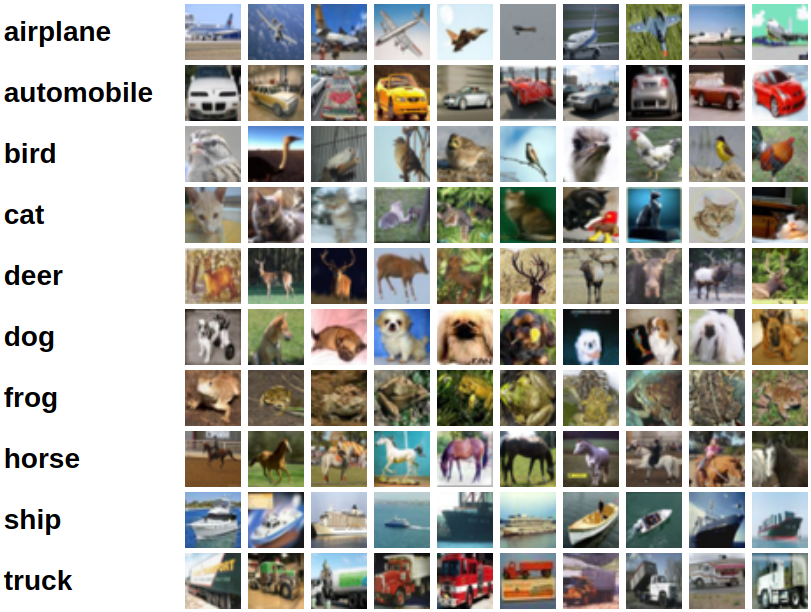
\includegraphics[width=0.7\textwidth]{figs/fig-2.png}
			\caption{The CIFAR-10 dataset}
		\end{figure}
	
		\item {\textbf{What kind of pre-processing might you consider doing?}}
		\par{Each training batch is a $ 10000\times3072 $ numpy array. Each row of the array stores a $ 32\times32 $ colour image. The first 1024 entries contain the red channel values, the next 1024 the green, and the final 1024 the blue. The value of each channel is between $ [0, 255] $. We are going to scale the RGB channel from $ [0, 255] $ to $ [0, 1] $. By standardizing the data, we could train faster and reduce the chance of getting stuck in a local optima.}
	\end{enumerate}
	\item {\textbf{Our Model:}} 
	\begin{figure}[H]
		\centering
		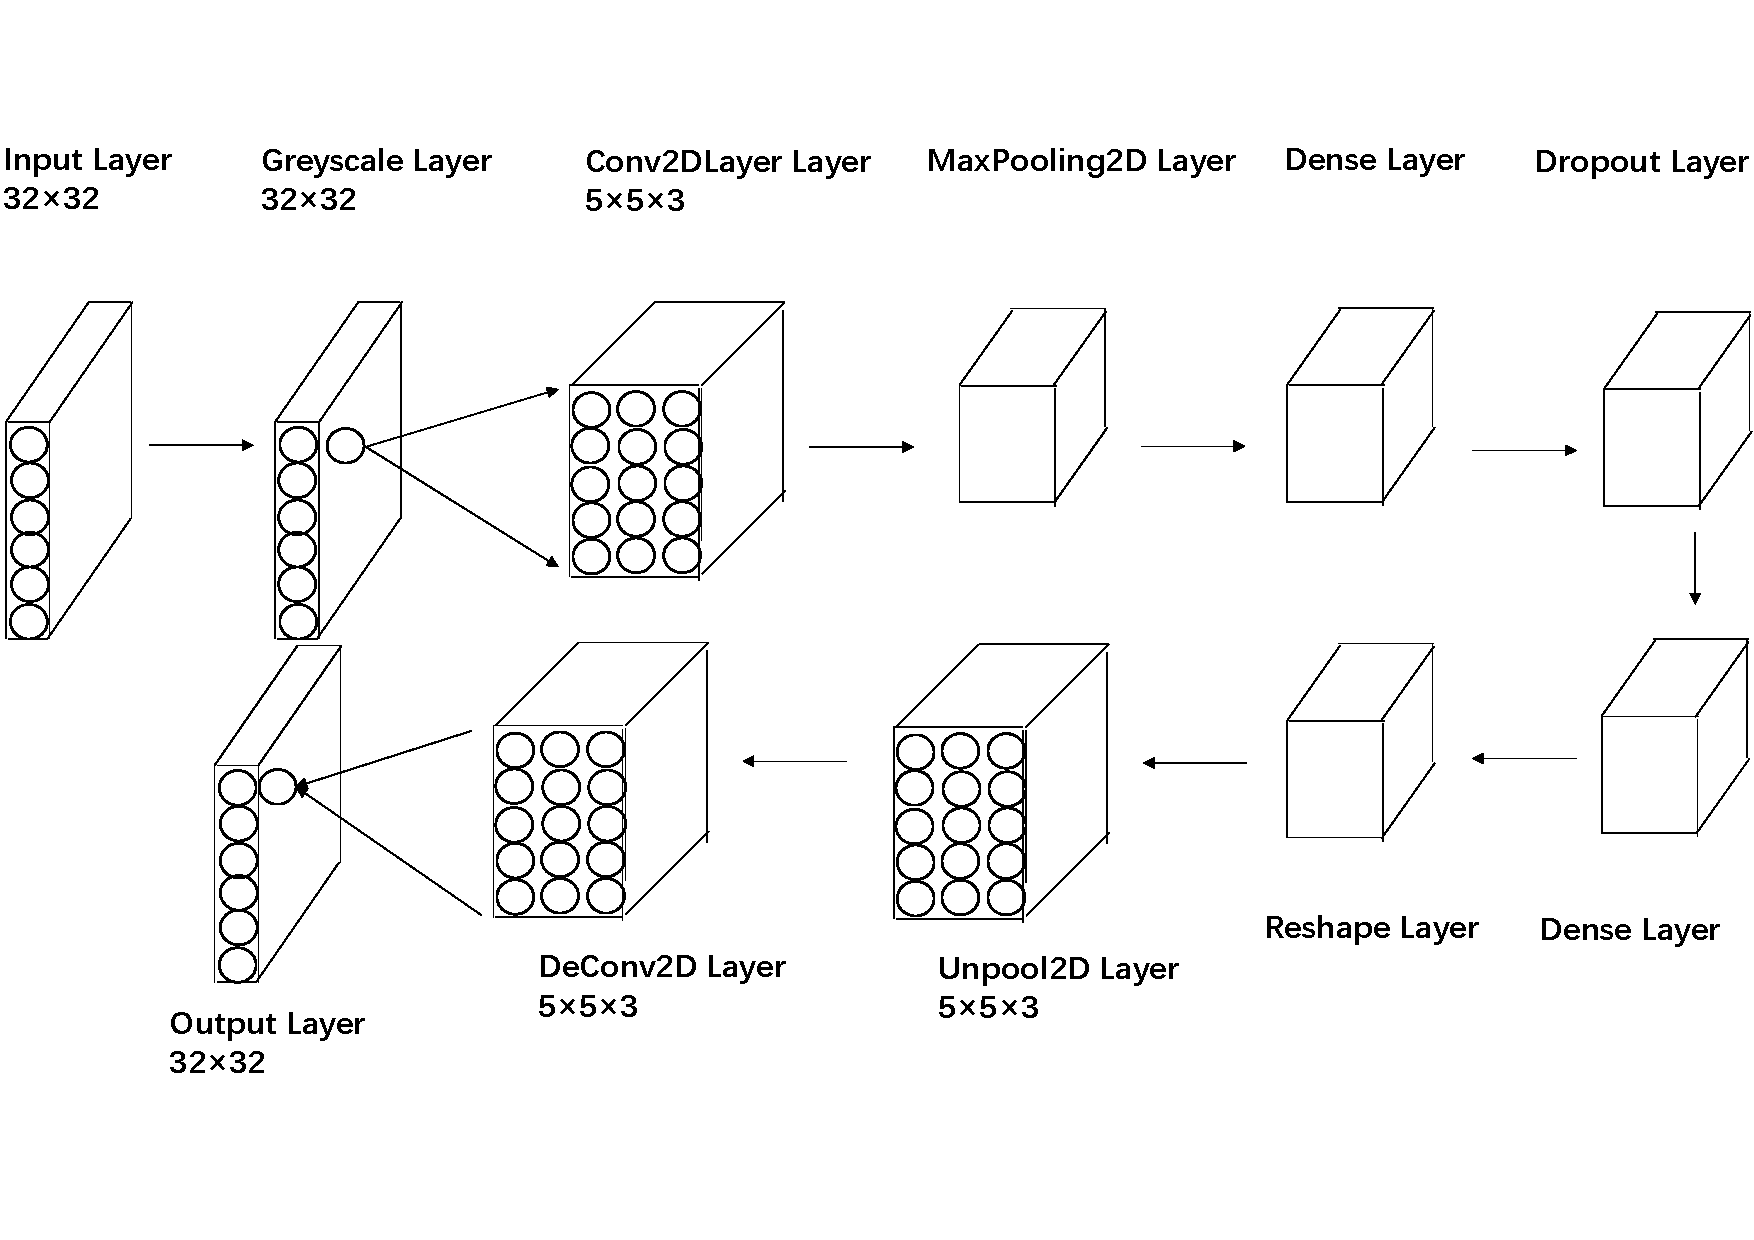
\includegraphics[width=.8\textwidth]{figs/structure.pdf}
		\caption{Our model}
	\end{figure}
	\par{1.	Input layer, use 4d-tensor to represent the input image.
	}\par{2.	Greyscale layer, calculates the greyscale of the input colored image.
	}\par{3.	Conv2D layer, in this layer we are using a filter of size 5*5*3(5 pixels width an height, and 3 because images have depth 3, the color channels). During the forward pass, we convolve each filter across the width and height of the input volume and compute dot products between the entries of the filter and the input at any position. In this process, we will produce a 2-d activation map that gives the responses of that filter at every spatial position. Intuitively, the network will learn filters that activate when they see some type of visual features, such as an edge of some orientation or a blotch of some color on the first layer, or eventually some wheel-like patterns on higher layers of the network. We will stack these activation maps along the depth dimension and produce the output volume.
	}\par{4.	MaxPool2DLayer, this layer’s function is to progressively reduce the spatial size of the representation to reduce the amount if parameters and computation in the network, and hence to also control overfitting. This layer operates independently on every depth slice of the input and resizes it spatially, using the MAX operation.
	}\par{5.	Dense layer, in this layer the neurons have full connections to all activations in the previous layer. Their activations can hence be computed with a matrix multiplication followed by a bias offset.
	}\par{6.	Dropout layer, this layer is a regularizer that randomly sets input values to zero. It can be used to prevent overfitting.
	}\par{7.	A Dense layer and a Reshape layer, these two layers serve as preparation for the Unpool2D layer.
	}\par{8.	Unpool2D Layer, this layer performs unpooling over the last two dimensions of a 4D tensor. This layer is essential if we want to reconstruct the image.
	}\par{9.	Deconvolution layer. This layer is used for upsampling (backwards strided convolution). It can coarse outputs to dense pixels by interpolation. In-network upsampling is fast and effective for learning dense prediction.
	}\par{10.	Output layer, this layer reshapes the network and outputs the generated image.
	}
	\item {\textbf{Evaluating the Model:}} 
	\begin{enumerate}
		\item {\textbf{Given a model for moving from grayscale images to color images (whatever spaces you are mapping between), how can you evaluate how good your model is?}}
		\par{For the evaluation part, we used the squared loss as the criteria. \[ \mathcal{L} = || output - input ||^2 \] When the loss is small enough, we can know our model is performing good.}
		\item {\textbf{How can you assess the error of your model (hopefully in a way that can be learned from)? }}
		\begin{itemize}
			\item {From the numerical perspective, the mean squared validation loss is, the better the model is performing. }
			\item {From the perceptual perspective, the closer the color is to the original picture, the better the model is performing.}
		\end{itemize}
	\end{enumerate}
	\item {\textbf{Training the Model:}} 
	\begin{enumerate}
		\item{Representing the problem is one thing, but can you train your model in a computationally tractable manner?}
		\par{It is actually quite easy to train our model because of the small size of the input. Generally, for each iteration, we would need to train for 40 seconds using a GTX 1070ti, for 25 seconds using a GTX 1080ti. We could achieve a good result in less than 100 iterations of training most of the time.}
		\item{What algorithms did you draw on?}
		\par{We are using Stochastic Gradient Descent algorithm with Nestrerov momentum, and we are using back propagation to update the gradient.}
		\item{How did you determine convergence?}
		\par{We validate the model and print out the validation loss every 10 iterations. When the validation loss stabilizes and even starts to rise, we stop our training and call it a convergence.}
		\item{How did you avoid overfitting?}
		\par{We are using Max Pooling layers and Dropout Layers in our model to prevent overfitting.}
		\begin{itemize}
			\item {Max pooling is basically selecting a subset of features, so we are less likely to be always training on false patterns.}
			\item {Dropout layers randomly drop some components of our neural network with some probability, which actually creates a different network. Thus after we finished the training, we actually have an ensemble of models. The probability is typically 50\%, but after our experiments, we found 30\% is better.}
		\end{itemize}
	\end{enumerate}
	\item {\textbf{Assessing the Final Project:}} 
	\begin{enumerate}
		\item {How good is your final program, and how can you determine that? How
			did you validate it?}
		\begin{figure}
			\centering
			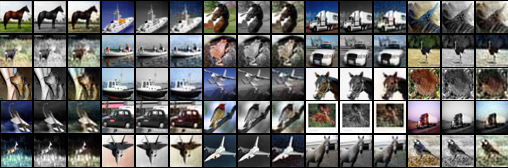
\includegraphics[width=\textwidth]{figs/fig-5.png}
			\caption{Some results}
			\label{fig-5}
		\end{figure}
		\par{Our final model is satisfying as Fig \ref{fig-5} shows.}
		\par{We use our validation dataset to calculate the validation loss. The validation loss of our final model achieved 20.928495, which is reasonable to us. }
		\item {What is your program good at, and what could use improvement?}
		\item {Do your program's mistakes `make sense'?}
		\begin{figure}[H]
			\centering
			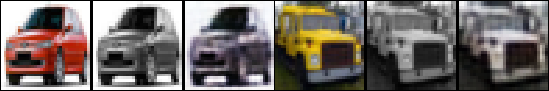
\includegraphics[width=0.7\textwidth]{figs/fig-3.png}
			\caption{Some results}
			\label{fig-3}
		\end{figure}
		\par{The colorizer can totally mess up blue and red or white and yellow as Fig \ref{fig-3} shows. But to be honest, we cannot tell the color of the car by just looking at its grayscale image. We think this kind of mistakes are quite resonable.}
		\item {What happens if you try to color images unlike anything the program was trained on?}
		\item {What kind of models and approaches, potential improvements and fixes, might you consider if you had more
			time and resources?}
	\end{enumerate}
\end{itemize}

\section{Our understanding towards CNN}
\par{Please refer to toyCNN/docs/Usage.html and toyCNN/docs/HowToBuildACNN.html. Thank you!}

\end{document}